Cassandra \cite{will10} was created by Facebook and is based on Dynamo \cite{Hastorun2007} and BigTable \cite{Chang2008}. The main goals of this system have been, from scratch, to be highly scalable, decentralized and fault tolerant.

Eric Brewer's CAP theorem \cite{Brewer2000} states that it is impossible for a distributed computer system to simultaneously provide all three of the following guarantees:
\begin{itemize}
	\item Consistency
	\item Availability
	\item Partition Tolerance
\end{itemize}

The NoSQL implementations, including Cassandra, focus on the last two, relaxing the consistency guarantee, providing eventual consistency. Usually, NoSQL members are key-value stores, that have nearly no structure in their data model, apart from what can be seen as an associative array. On the other hand, Cassandra is a column oriented database system, with a rather complex data model, that is described below.

Cassandra is built to optimize reads, therefore it does no processing when fetching the stored data. All the processing, as sorting, indexing (column families can be used to create indexes), and so on, is done when storing the said data, which is basically the opposite of what happens on the classical models (\ac{rdbms}).

\section{Data Model}
In this section the data model of Cassandra \cite{sarkissian09} will be explained from the most basic component to the most complex, with some detail, since this is very different from the relational data model most people are used to, and takes some time to digest and understand.

The basic building block of Cassandra are columns (Fig. \ref{fig:column}), that consist of a tuple with three elements, a name, a value and a timestamp.

\begin{figure}[htb]
  \begin{center}
    \leavevmode
    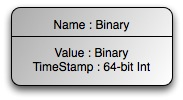
\includegraphics[width=0.3\textwidth]{images/column.jpg}
  \end{center}
  \caption{Cassandra Column}
  \label{fig:column}
\end{figure}

In the next level of complexity there is the SuperColumn (Fig. \ref{fig:supercolumn}), that is also a tuple, but only has two elements, the name and the value with the particularity that the value is a map of keys to columns (this key has to be the same as the column's name).

\begin{figure}[htb]
  \begin{center}
    \leavevmode
    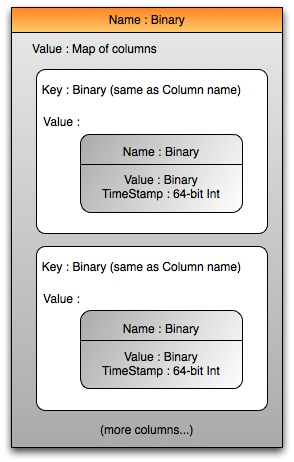
\includegraphics[width=0.4\textwidth]{images/supercolumn.jpg}
  \end{center}
  \caption{Cassandra SuperColumn}
  \label{fig:supercolumn}
\end{figure}

The maximum level of complexity is achieved with the Column Families, which ``glue'' this whole system together, it is a structure that can keep an infinite number of rows (super columns), and has a name, and a map of keys to rows as shown in picture \ref{fig:columnfamily}. Every operation under a single row key is atomic per replica, despite the number of columns affected.

Applications can specify the sort order of columns within a column family, that can be based on the name or on the timestamp. The system allows for multiple keyspaces (tables), but almost all deployments have only one in their schema.

\begin{figure}[!htb]
  \begin{center}
    \leavevmode
    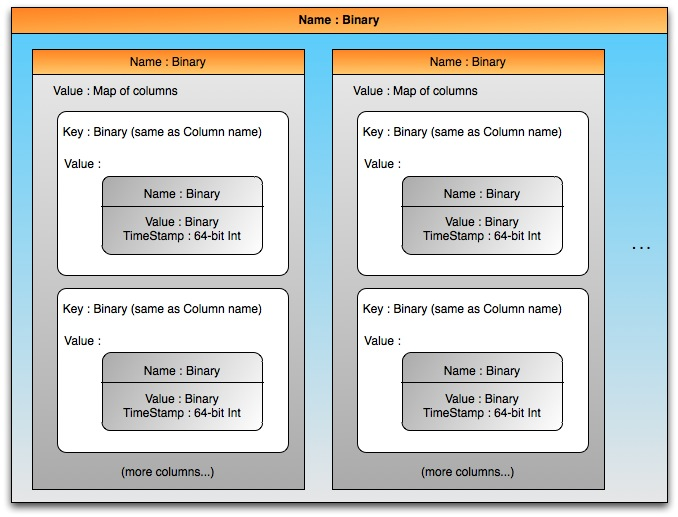
\includegraphics[width=0.8\textwidth]{images/columnfamily.jpg}
  \end{center}
  \caption{Cassandra ColumnFamily}
  \label{fig:columnfamily}
\end{figure}

There is a variation of ColumnFamilies that are SuperColumnFamilies. The only difference is that where a ColumnFamily has SuperColumns with maps of columns, a SuperColumnFamily has SuperColumns with maps of SuperColumns. 

\section{Querying}
Cassandra's \ac{api} is what defines it's querying capabilities, and consists of three simple methods \cite{lakshmanMalik}:

\begin{itemize}
	\item \emph{insert(table, key, rowMutation)}
	\item \emph{get(table, key, columnName)}
	\item \emph{delete(table, key, columnName)}
\end{itemize}	

In the method signatures above, \emph{columnName} can refer to a specific column in a column family, a column family, simple or super, or a column in a supercolumn. The \emph{rowMutation} specifies the changes to the row in case it was already there, or the row to be added.

\section{Consistency}
Cassandra allows clients to specify the desired consistency level on reads and writes, based on the replication factor previously defined in a configuration file, present in every cluster. Notice that if R + W > Replication Factor, where R is the number of nodes to block for on read, and W the ones to block for on write, the most consistent behavior will be achieved\footnote{Because the repair replication process only requires a write to reach a single node to propagate, a write which ``fails'' to meet consistency requirements will still appear eventually as long as it was written to at least one node.}.\\

Cassandra uses replication to achieve high availability and durability. Each data item is replicated at N nodes, where N is the afore mentioned replication factor, assigning each key to a coordinator node (chosen through consistent hashing\footnote{``Consistent hashing is a scheme that provides hash table functionality in a way that the addition or removal of one slot does not significantly change the mapping of keys to slots. By using consistent hashing, only K/n keys need to be remapped on average, where K is the number of keys, and n is the number of slots.'' in Wikipedia, 13/12/2010}), that in addition to storing locally each key within his range, replicates these keys at the N-1 nodes in the consistent hashing ring. 

Cassandra system elects a leader amongst its nodes using Zookeeper \cite{Junqueira2007}, that is contacted by all joining nodes, and tells them for what ranges they are responsible. The leader also makes an effort for maintaining the invariant that no node is responsible for more than N-1 ranges in the ring. 

In Cassandra every node is aware of every other node in the system and, therefore the range they are responsible for.
